\documentclass{beamer}
\usecolortheme{beaver}
\beamertemplatenavigationsymbolsempty
\setbeamertemplate{blocks}[rounded=true, shadow=true]
\setbeamertemplate{footline}[page number]
\setbeamertemplate{caption}{\raggedright\insertcaption\par}

\usepackage[utf8]{inputenc}
\usepackage[english, russian]{babel}
\usepackage{amssymb,amsfonts,amsmath,mathtext}
\usepackage{array}
\usepackage{multicol}
\usepackage{hhline}
\usepackage{multirow}
\usepackage{graphicx}
\graphicspath{{../figures/}}
\usepackage{tikz}
\usetikzlibrary{shapes.geometric,arrows.meta,positioning}

\title[Обратные задачи в моделировании nPDE]
{Обратные задачи в моделировании нейронных дифференциальных уравнений в частных производных}

\author[А. Терентьев]
{Александр Терентьев}

\institute[МФТИ]
{
    Московский физико-технический институт \\
    Физтех-школа прикладной математики и информатики \\
    Кафедра интеллектуальных систем \\
    Научный руководитель: д.ф.-м.н. Стрижов Вадим Викторович
}

\begin{document}

\frame{\titlepage}

\begin{frame}
\frametitle{Цель исследования}
\begin{block}{Проблема}
В задачах EEG трудность вызывает получение точного сигнала от головного мозга. Исследователи встречаются со следующими проблемами. 
Высокая чувствительность прибора к движениям и тремору, обусловленному психоэмоциональным напряжением пациента, вызывает помехи в работе, что может затруднить диагностику. 
\end{block}
\begin{block}{Цель}
Целью работы является предложить метод решения обратной задачи для уравнений в частных производных,  обеспечивая более точные и устойчивые результаты по сравнению 
с существующими методами и выполняющие физичесмкие ограничения.
\end{block}

\end{frame}

\begin{frame}
\frametitle{Постановка обратной задачи ДУЧП}

\begin{block}{Операторная формулировка}
Пространства: $\mathcal{S}$ ~-- гильбертово пространство распределений поляризации, 
$\mathcal{F}$ ~-- гильбертово пространство потенциалов, $\mathcal{O} = \mathbb{R}^n$ ~-- пространство наблюдений 
на $n$ датчиках.

Оператор наблюдения $K$ задаётся композицией оператора потенциала $T$ и оператора измерения $C$:
\begin{equation}
    T: \mathcal{S} \to \mathcal{F}, \quad C: \mathcal{F} \to \mathcal{O}, \quad K = C \circ T.
\end{equation}

Оператор $T$ линеен, ограничен и положительно определён, оператор $C$ линеен и ограничен.

Наблюдаемые данные $d \in \mathcal{O}$, шум $\eta \in \mathcal{O}$ и искомые источники $s$ связаны уравнением:
\begin{equation}
    d = K s + \eta
\end{equation}
\end{block}

\end{frame}

\begin{frame}
\frametitle{Уравнения Максвелла в операторной постановке}
Оператор $T: \mathcal{S} \to \mathcal{F}$ определяется как $T\mathbf{P} = (\phi, \mathbf{A})$, где $\phi$ и $\mathbf{A}$ --- решения волновых уравнений:

Плотность заряда и тока:
\begin{equation}
    \rho = -\operatorname{div} \mathbf{P}, \quad \mathbf{j} = \frac{\partial \mathbf{P}}{\partial t}.
\end{equation}
Уравенения Максвелла для потенциалов:
\begin{equation}\label{eq:maxwell}
    \square \phi = 4\pi \nabla \cdot \mathbf{P},
    \square \mathbf{A} = -\frac{4\pi}{c} \frac{\partial \mathbf{P}}{\partial t}, 
\end{equation}

где $\square = \nabla^2 - \frac{1}{c^2} \frac{\partial^2}{\partial t^2}$ ~-- оператор Д’Аламбера.

Калибровка Лоренца:
\begin{equation}
    \nabla \cdot \mathbf{A} + \frac{1}{c} \frac{\partial \phi}{\partial t} = 0.
\end{equation}



\end{frame}

\begin{frame}
\frametitle{Регуляризация обратной задачи}

\begin{block}{Регуляризованный функционал}
\begin{equation}
    J(s) = \|K s - d\|^2 + \alpha \langle T s, s \rangle + \beta \mathrm{TV}(s).
\end{equation}

Энергетический регуляризатор:
\begin{equation}
    \langle T s, s \rangle = \int_{\Omega} (\rho \phi + \mathbf{A} \cdot \mathbf{j}) \, d\mathbf{r} > 0.
\end{equation}
\end{block}

\end{frame}

\begin{frame}
\frametitle{Теорема о единственности решения}

\begin{block}{Постановка}
Пусть $\mathcal{S}, \mathcal{F}$ --- гильбертовы пространства, $\mathcal{O} = \mathbb{R}^n$, $T: \mathcal{S} \to \mathcal{F}$ --- положительно определённый оператор, $C: \mathcal{F} \to \mathcal{O}$ --- ограниченный оператор наблюдения, $\mathrm{TV}: \mathcal{S} \to [0,+\infty]$ --- выпуклый функционал, $\alpha > 0$, $\beta \geq 0$.
\end{block}

\begin{block}{Функционал}
\begin{equation}
    J(s) = \|C T s - d\|_{\mathcal{O}}^2 + \frac{\alpha}{2} \langle T s, s \rangle_{\mathcal{S}} + \beta \mathrm{TV}(s).
\end{equation}
\end{block}

\begin{block}{Утверждение}
Функционал $J(s)$ строго выпукл и имеет единственный глобальный минимум $s^* \in \mathcal{S}$.
\end{block}

\end{frame}

\begin{frame}
\frametitle{Теорема о сходимости минимизаторов}

\begin{block}{Постановка}
Пусть $\mathcal{S}, \mathcal{F}, \mathcal{O}$ --- гильбертовы пространства, 
$T, T_n: \mathcal{S} \to \mathcal{F}$ --- ограниченные линейные операторы, 
$C: \mathcal{F} \to \mathcal{O}$ --- ограниченный оператор наблюдения, 
$T$ положительно определён, $\mathrm{TV}: \mathcal{S} \to [0,+\infty]$ --- полная вариация, 
$\alpha > 0$, $\beta \geq 0$,
$T_n \to T$ равномерно на ограниченных множествах.
\end{block}

\begin{block}{Функционалы}
\begin{align}
    J(s) &= \|C T s - d\|_{\mathcal{O}}^2 + \frac{\alpha}{2} \langle T s, s \rangle_{\mathcal{S}} + \beta \mathrm{TV}(s), \\
    J_n(s) &= \|C T_n s - d\|_{\mathcal{O}}^2 + \frac{\alpha}{2} \langle T_n s, s \rangle_{\mathcal{S}} + \beta \mathrm{TV}(s).
\end{align}
\end{block}

\begin{block}{Утверждение}
Тогда минимизаторы $s_n^* = \arg\min J_n(s)$ сходятся к минимизатору $s^* = \arg\min J(s)$ сильно в $\mathcal{S}$ при $n \to \infty$.
\end{block}

\end{frame}

\begin{frame}
\frametitle{Метод: Time-Aware нейросеть и суммарный функционал}

\begin{columns}[T]
\column{0.52\textwidth}

\begin{tikzpicture}[
    every node/.style={font=\tiny},
    box/.style={draw, rounded corners=2pt, minimum width=1.1cm, minimum height=0.38cm,
                align=center, fill=white},
    inputbox/.style={box, fill=red!15},
    hidbox/.style={box, fill=blue!12},
    outbox/.style={box, fill=green!20},
    concatbox/.style={box, fill=orange!20, minimum width=2.3cm},
    arr/.style={-Stealth, thick, gray!70},
    scale=0.82, transform shape
]

% --- Inputs ---
\node[inputbox] (xyz)  at (0,0)    {$(x,y,z)$};
\node[inputbox] (t)    at (2.4,0)  {$t$};

% --- Spatial branch ---
\node[hidbox] (s1) at (0, -0.9) {FC-6, ReLU};
\node[hidbox] (s2) at (0, -1.8) {FC-8, ReLU};

% --- Temporal branch ---
\node[hidbox] (fe)  at (2.4, -0.9) {Fourier\\$\sin(kt),\cos(kt)$};
\node[hidbox] (t1)  at (2.4, -1.8) {FC-16, ReLU};
\node[hidbox] (t2)  at (2.4, -2.7) {FC-6, ReLU};

% --- Concat ---
\node[concatbox] (cat) at (1.2, -3.6) {Concat};

% --- Joint branch ---
\node[hidbox, minimum width=2.3cm] (j1) at (1.2,-4.5) {FC-32, ReLU};
\node[hidbox, minimum width=2.3cm] (j2) at (1.2,-5.4) {FC-16, ReLU};
\node[hidbox, minimum width=2.3cm] (j3) at (1.2,-6.3) {FC-8,  ReLU};

% --- Output ---
\node[outbox, minimum width=2.3cm] (out) at (1.2,-7.1)
    {$\phi,A_x,A_y,A_z,P_x,P_y,P_z$};

% --- Arrows ---
\draw[arr] (xyz) -- (s1);
\draw[arr] (s1)  -- (s2);
\draw[arr] (s2)  -- (cat);

\draw[arr] (t)   -- (fe);
\draw[arr] (fe)  -- (t1);
\draw[arr] (t1)  -- (t2);
\draw[arr] (t2)  -- (cat);

\draw[arr] (cat) -- (j1);
\draw[arr] (j1)  -- (j2);
\draw[arr] (j2)  -- (j3);
\draw[arr] (j3)  -- (out);

% --- Branch labels ---
\node[font=\tiny\itshape, gray] at (-0.85,-1.35) {простр.};
\node[font=\tiny\itshape, gray] at (3.55,-1.8)   {врем.};

\end{tikzpicture}

\column{0.46\textwidth}

{\footnotesize\textbf{Суммарный функционал:}}

\begin{block}{\footnotesize nPDE Loss}
{\scriptsize Невязка Д'Аламбера: $\square\phi = 4\pi\nabla\!\cdot\!\mathbf{P}$,\; $\square\mathbf{A} = -\tfrac{4\pi}{c}\partial_t\mathbf{P}$}
\end{block}

\vspace{-3pt}
\begin{block}{\footnotesize BC Loss}
{\scriptsize Граничные условия (Дирихле / PML):}\\
{\scriptsize $\mathcal{L}_{\mathrm{BC}} = \|\phi|_\Gamma\|^2 + \|\mathbf{A}|_\Gamma\|^2$}
\end{block}

\vspace{-3pt}
\begin{block}{\footnotesize Data Loss (барьерная)}
{\scriptsize Соответствие данным ЭЭГ:}\\
{\scriptsize $\mathcal{L}_{\mathrm{data}} = \lambda_d(\|Ks-d\|^2 + \alpha_d\|Ks-d\|^4)$}
\end{block}

\vspace{-3pt}
\begin{block}{\footnotesize Регуляризация}
{\scriptsize Энергетический и TV-члены:}\\
{\scriptsize $\mathcal{L}_{\mathrm{reg}} = \alpha\langle Ts,s\rangle + \beta\,\mathrm{TV}(s)$}
\end{block}

\vspace{2pt}
{\scriptsize
$\mathcal{L} = \mathcal{L}_{\mathrm{PDE}} + \mathcal{L}_{\mathrm{BC}} + \mathcal{L}_{\mathrm{data}} + \mathcal{L}_{\mathrm{reg}}$}

\end{columns}
\end{frame}

\begin{frame}
\frametitle{Экспериментальные данные}

\begin{block}{Реальные данные (Brunton et al.)}
Записи ЭЭГ 13 испытуемых при выполнении когнитивных и моторных задач. Данные предобработаны:
\begin{enumerate}
    \item Частота дискретизации: 250 Гц.
    \item Фильтрация: полоса 1–50 Гц.
    \item Удаление артефактов: метод ICA.
    \item Нормализация амплитуды сигнала.
\end{enumerate}
\end{block}

\begin{block}{Синтетические данные}
Модель овальной головы с 16 датчиками и 2 источниками сигнала:
\begin{enumerate}
    \item Частота дискретизации: 50 Гц.
    \item Геометрия: овальная оболочка головы с внутренними источниками.
    \item Контролируемый уровень шума.
\end{enumerate}
\end{block}

\end{frame}



\begin{frame}
\frametitle{Визуализация синтетической модели}

\begin{figure}[h]
\centering
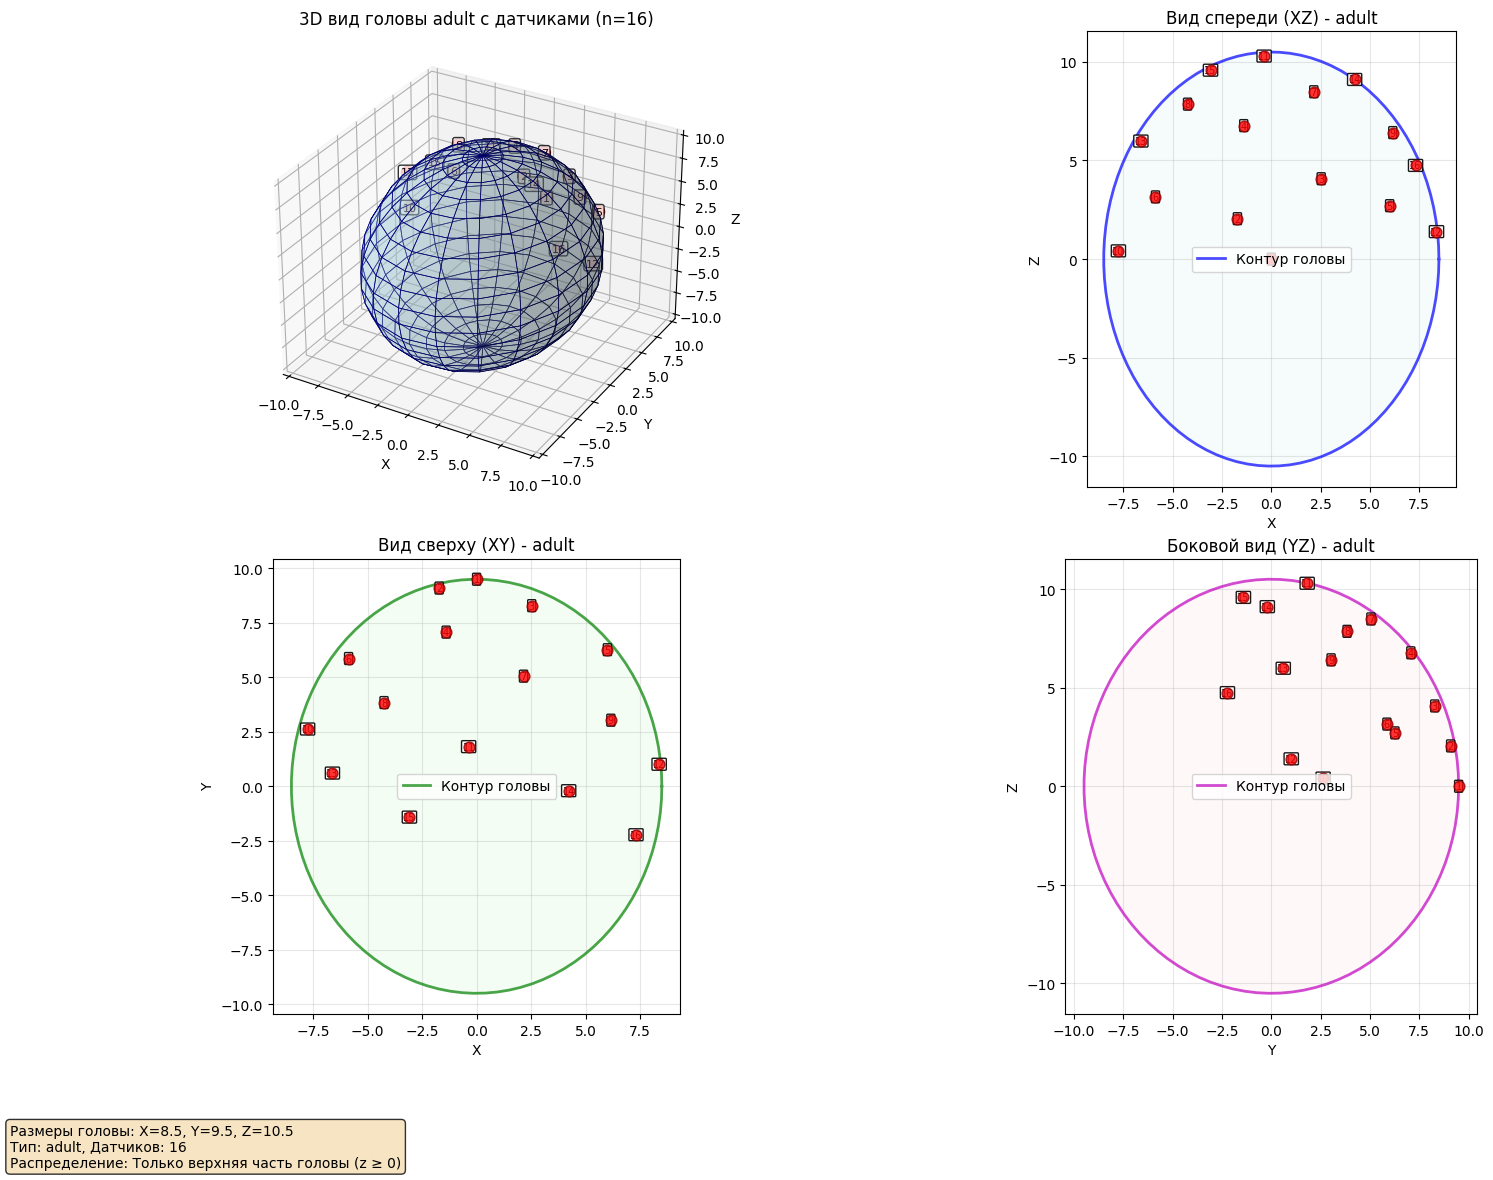
\includegraphics[width=0.6\textwidth]{synthetic_head_views.png}
\caption{Синтетическая модель головы с датчиками.}
\end{figure}

\end{frame}

\begin{frame}

\frametitle{Визуализация восстановленния источников}

\begin{figure}[h]
\centering
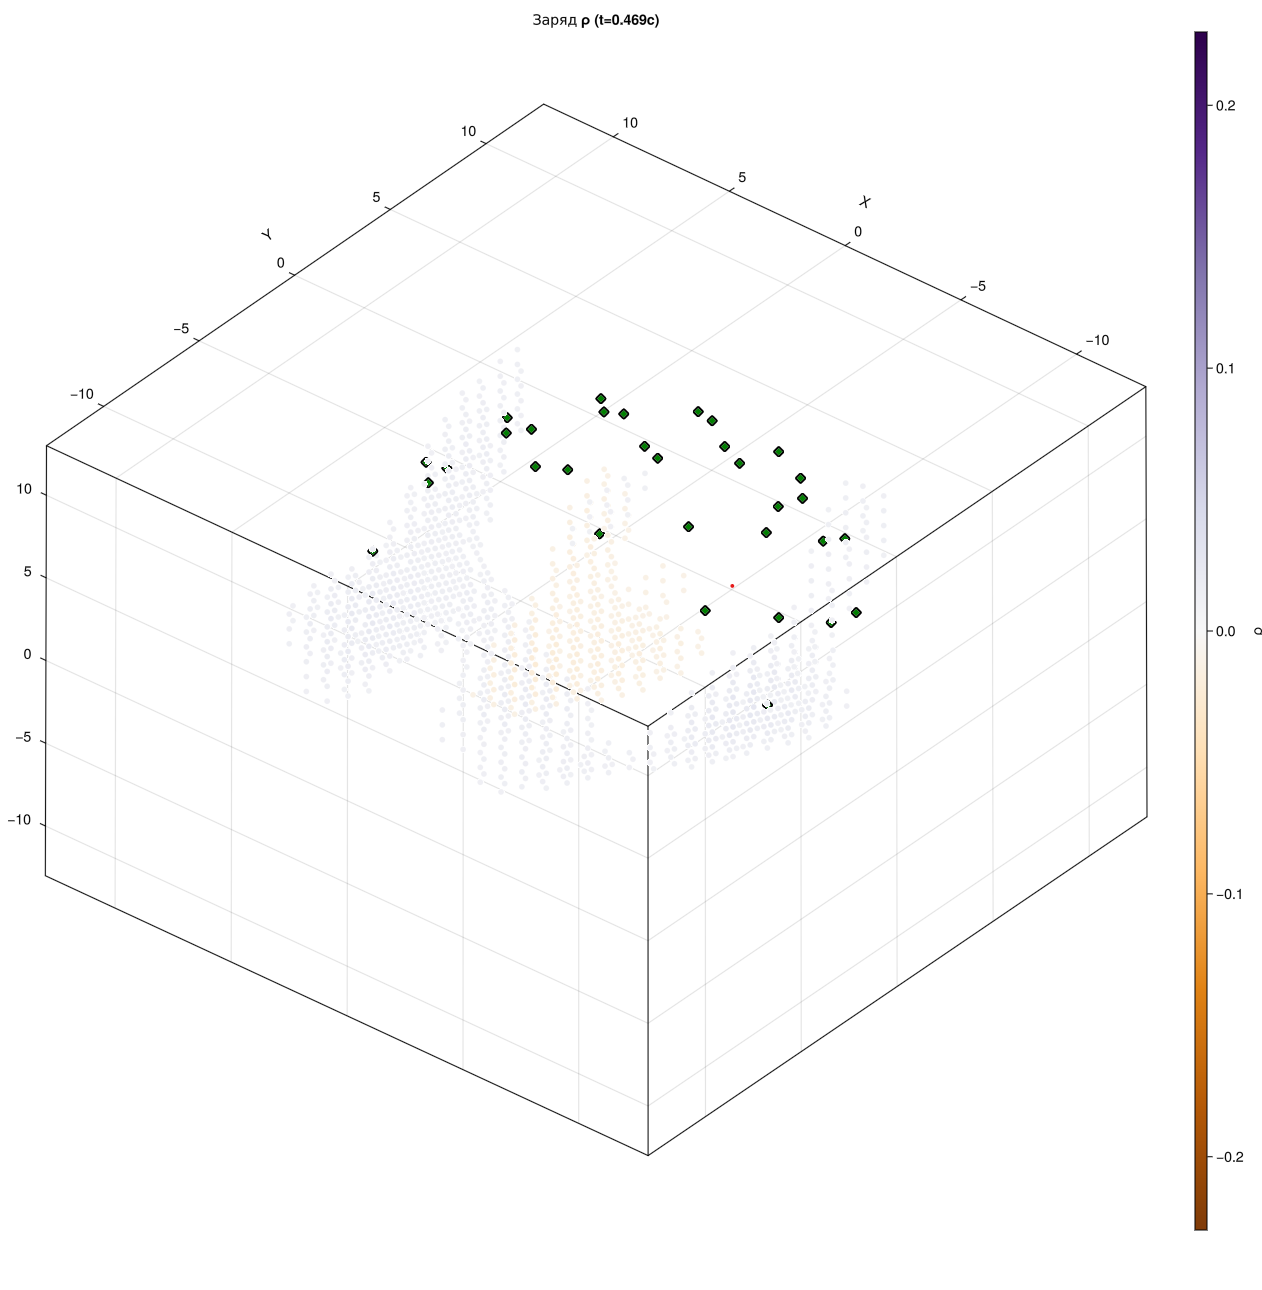
\includegraphics[width=0.6\textwidth]{head_rho.png}
\caption{Результат воостановления источника.}
\end{figure}

\end{frame}

\begin{frame}
\frametitle{Экспериментальные результаты}

\begin{block}{Датасет Brunton et al.}
\begin{table}[h]
\centering
\begin{tabular}{lc}
\hline
Метод & Sensor MSE \\
\hline
Предложенный метод & $0.11 \pm 0.017$\\
LORETA & $0.15 \pm 0.012$\\
\hline
\end{tabular}
\end{table}
\end{block}

\begin{block}{Синтетические данные}
\begin{table}[h]
\centering
\begin{tabular}{lcc}
\hline
Метод & Sensor MSE & Deep MSE \\
\hline
Предложенный метод & $0.050 \pm 0.004$ & $0.38 \pm 0.03$ \\
LORETA & $0.071 \pm 0.003$ & $0.47 \pm 0.01$ \\
\hline
\end{tabular}
\end{table}
\end{block}

\end{frame}

\begin{frame}

\frametitle{Выносится на защиту}

\begin{enumerate}
    \item Разработан метод обратной задачи уравнений в частной производной в операторной постановке.
    \item Доказательство линейности и ограниченности оператора $T$ для уравнений Максвелла.
    \item Регуляризованный функционал с энергетическим членом и $\mathrm{TV}(s)$.
    \item Теоремы о сходимости минимизаторов и единственности решения.
    \item Экспериментальное подтверждение эффективности метода на основе задачи ЭЭГ.
\end{enumerate}

\end{frame}

\end{document}